\todo[inline]{Beskriv antagelse om at spillets aktiver er propritære (og ikke open-source, som de faktisk er nu grundet nemhedens skyld)}
\todo[inline]{Prisovervejelser}
\todo[inline]{Platformovervejelser}
\todo[inline]{Lanceringskampagne}
\todo[inline]{Fremtidige opdateringer}
\todo[inline]{Early Access-development (versus ``gammeldags'' udvikling [golden edition])}
Spilvirksomheder udgiver sjældent et spil 100\% første gang. Man taler ofte om ``The software release life cycle'' — denne beskriver udviklings-, test- og distribueringsfaserne af et stykke software.\footfullcite{softwareRelease}

\begin{figure}[H]
    \centering
    \fbox{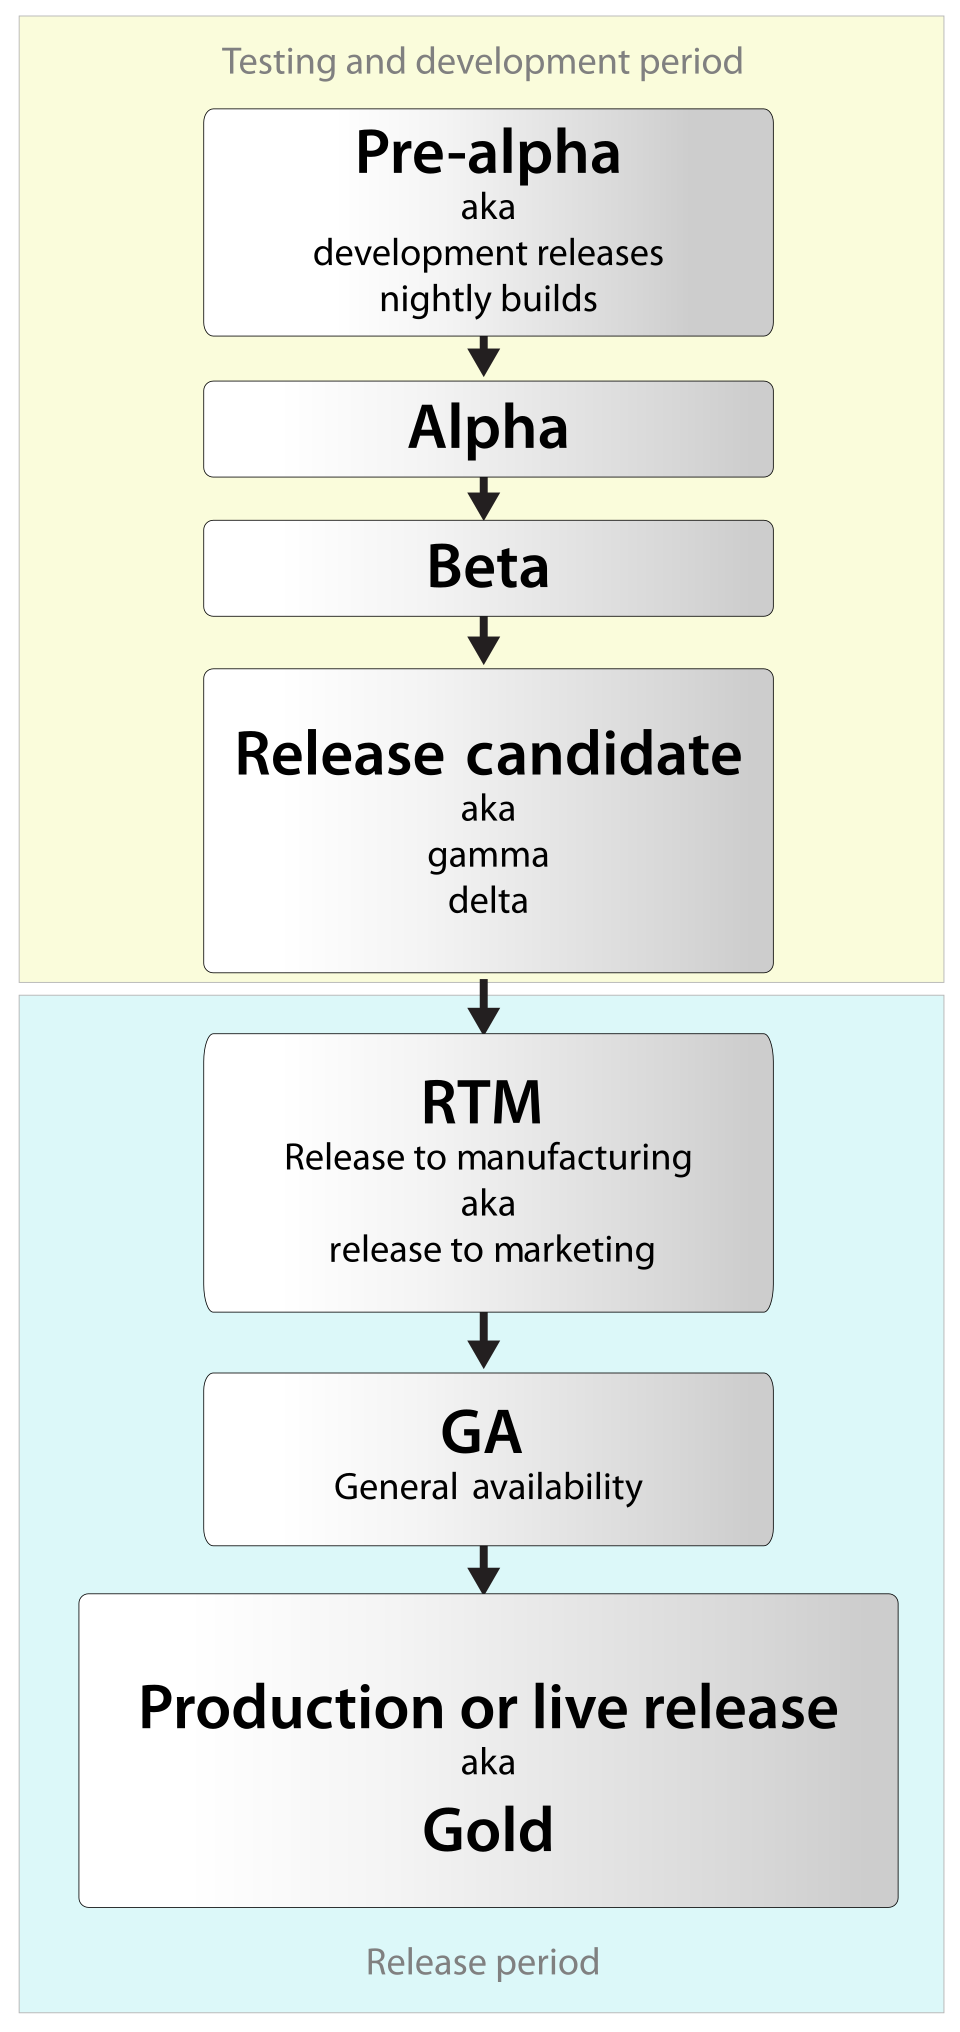
\includegraphics[width=0.5\linewidth]{assets/release_cycle.png}}
    \caption{Et eksempel af: ``software release life cycle''\cite{softwareRelease}}
    \label{fig:release_cycle}
\end{figure}

I den traditionelle udviklingsmodel — ofte kaldet \textit{golden edition}-modellen — udgives 
spillet først når det er færdigudviklet og gennemtestet. Spillet betragtes som låst 
(\textit{gold}) når det er klar til distribution, og efterfølgende opdateringer er forbeholdt fejlrettelser. Denne model stiller høje krav til forudgående planlægning, da det er svært at ændre fundamentale designbeslutninger efter udgivelsen. 
Før i tiden, da man købte spil i fysiske udgaver på CD eller kassette, må det siges at have været ret svært at opdatere spillet efterfølgende for alle ens kunder, hvis man lige skulle rette en lille fejl. Med internettets udbredelse og digitale distributionsplatforme som Steam mistede golden edition-modellen sin praktiske nødvendighed — det blev pludselig trivielt at sende opdateringer ud til alle spillere på én gang, hvilket banede vejen for mere iterative udviklingsmodeller som Early Access.

En nyere, og i dag meget udbredt alternativ model er \textit{Early Access}. Early Access er  hvor spillet udgives i en ufærdig tilstand (ofte til en reduceret pris). Spillerne får dermed adgang til spillet tidligt i udviklingsforløbet og bidrager aktivt til dets forbedring gennem feedback og stress test af systemer. Denne model er særligt populær inden for uafhængigt producerede spil (indie-spil), hvor udviklerne ikke nødvendigvis har ressourcer til en fuldstændig færdigudviklet udgivelse. Velkendte eksempler på spil der benyttede Early Access er \textit{Minecraft} og \textit{Satisfactory}.

The software release cycle består af to hovedfacer delt op i 7 stadier. Den første face er test- og udviklingsfacen, herunder er følgende stadier:
\begin{enumerate}
    \item \textbf{Pre-alpha}\\
    Pre-alpha er det første stadie et spil har. Dette stadie inkluderer alt før mere formel testing går i gang. Pre-alpha-versioner er ofte den version man har efter en dags udvikling.
    \item \textbf{Alpha}\\
    Alpha-stadiet betegner spillet når det stadig er i en intern testface, og altså endu ikke eksponeret for omverdnen. Alpha versioner har ofte mange ufuldkommne elementer, men stadig de centrale elementer begynder at tage form.
    \item \textbf{Beta}\\
    I beta-stadiet er spillet for det meste færdigt, det har ofte dog en helt masse ukendte/skjulte fejl som løbende bliver udbedret henimod den fulde version.
    \item \textbf{Release candidate}\\
    Release candidate (udgivelseskandidaten), er den beta-version med potentialet til at udgøre et stabilt produkt, altså et næsten fejlfrit produkt.
\end{enumerate}

Herefter overgår produktet til udgivnings facen (Release period)
\begin{enumerate}
    \item \textbf{RTM}\\
    RTM (\textit{Release to Manufacturing}) er det stadie hvor produktet erklæres færdigt og 
    sendes til produktion. Historisk set betød dette at spillet blev kopieret til fysiske medier 
    som CD'er eller kassetter klar til distribution — deraf navnet.
    \item \textbf{GA}\\
    GA (\textit{General Availability}) er det stadie hvor produktet bliver gjort tilgængeligt 
    for offentligheden. Det er på dette tidspunkt, at spillet kan købes og spilles af alle.
    \item \textbf{Production / Gold}\\
    Gold-stadiet betegner den endelige, stabile version af produktet. Spillet betragtes som 
    færdigt og låst — efterfølgende ændringer begrænses til kritiske fejlrettelser. Det er 
    denne model der kendetegner den klassiske \textit{golden edition}-udviklingsmodel.
\end{enumerate}


Skulle \textbf{SPIL NAVN} udgives kommercielt, ville Early Access-modellen være oplagt for os, da spillet stadig har ufuldkomndne features og ville kunne drage fordel af løbende brugerfeedback og økonomisk støtte i en tidlig fase.


\todo[inline]{Evt. regional prissættelse}
